\scanpage{120}
% archive foliation: 119
f) $1$ sommet d’ordre $3$, $1$ d’ordre $2$, $1$ d’ordre $2$
\figure{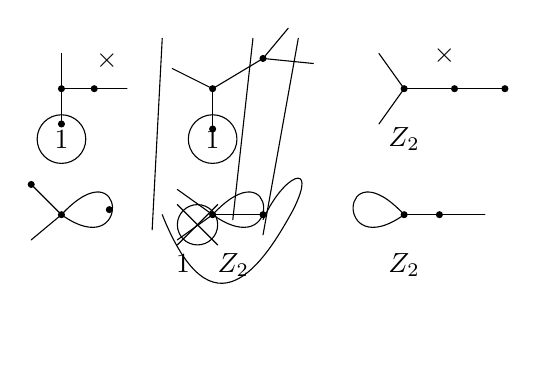
\begin{tikzpicture}[scale=.64,line cap=round,line join=round]\begin{scope}[shift={(0,1)}]\fill(0,0)circle(2pt);\draw(0,.7)--(0,-.7);\draw(0,0)--(1.3,0);\fill(0,-.7)circle(2pt);\fill(.65,0)circle(2pt);\node at(.9,.55){$\times$};\node[draw,circle]at(0,-1){$1$};\end{scope}\begin{scope}[shift={(3,1)}]\fill(0,0)circle(2pt);\draw(-.8,.4)--(0,0)--(1,.6)--(2,.5);\draw(0,0)--(0,-.8);\fill(0,-.8)circle(2pt);\fill(1,.6)circle(2pt);\draw(1,.6)--(1.5,1.2);\node[draw,circle]at(0,-1){$1$};\end{scope}\begin{scope}[shift={(6.8,1)}]\fill(0,0)circle(2pt);\draw(-.5,.7)--(0,0)--(-.5,-.7);\draw(0,0)--(2,0);\fill(1,0)circle(2pt);\fill(2,0)circle(2pt);\node at(.8,.65){$\times$};\node at(0,-1){$\mathbb Z_2$};\end{scope}\begin{scope}[shift={(0,-1.5)}]\fill(0,0)circle(2pt);\draw(0,0)..controls(1.3,1.4)and(1.4,-1)..(0,0);\draw(-.6,.6)--(0,0)--(-.6,-.5);\fill(-.6,.6)circle(2pt);\fill(.95,.1)circle(2pt);\end{scope}\begin{scope}[shift={(3,-1.5)}]\fill(0,0)circle(2pt);\draw(0,0)..controls(1.3,1.4)and(1.4,-1)..(0,0);\draw(-.7,.5)--(0,0)--(-.7,-.5);\draw(0,0)--(1,0);\fill(1,0)circle(2pt);\node at(0,-1){$\unsure{1}\quad\mathbb Z_2$};\end{scope}\begin{scope}[shift={(6.8,-1.5)}]\fill(0,0)circle(2pt);\draw(0,0)..controls(-1.3,1.4)and(-1.4,-1)..(0,0);\draw(0,0)--(1.6,0);\fill(.7,0)circle(2pt);\node at(0,-1){$\mathbb Z_2$};\end{scope}\draw(2,2)--(1.8,-1.8);\draw(3.8,2)--(3.4,-1.6);\draw(4.7,2)--(4,-1.9);\draw(2,-1.5)..controls(3,-4)and(4,-2.5)..(4.6,-1.4)..controls(5.1,-.4)and(4.4,-.7)..(4,-1.6);\draw(2.7,-1.7)circle(.4);\draw(2.3,-1.3)--(3.1,-2.1);\draw(3.1,-1.3)--(2.3,-2.1);\end{tikzpicture}}
\margin{$\left(\begin{smallmatrix}3\\2\\1\end{smallmatrix},\begin{smallmatrix}2_2\\1_2\end{smallmatrix},\unsure6\right)$\\$\left(\begin{smallmatrix}3\\2\\1\end{smallmatrix},\begin{smallmatrix}2_2\\1_2\end{smallmatrix},\unsure6\right)$\\$\left(\begin{smallmatrix}3\\2\\1\end{smallmatrix},\unsure{2_3},\begin{smallmatrix}5\\1\end{smallmatrix}\right)$\\$\left(\begin{smallmatrix}3\\2\\1\end{smallmatrix},2_3,\begin{smallmatrix}4\\2\end{smallmatrix}\right)$}
\figure{\begin{tikzpicture}\draw(0,0)..controls(.1,.7)and(.6,.8)..(.8,.8)--(.8,1.3);\draw(.9,.8)..controls(1.2,.4)and(2,.7)..(2.7,0);\draw(1.4,2.6)..controls(.8,2.4)..(1,2.1);\end{tikzpicture}}
g) $1$ sommet d’ordre $3$, \unsure{trois} d’ordre $1$
\figure{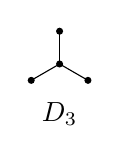
\begin{tikzpicture}[scale=.64,line cap=round,line join=round]\begin{scope}[shift={(0,0)}]\fill(0,0)circle(2pt);\draw(0,0)--(90:.65);\draw(0,0)--(210:.65);\draw(0,0)--(330:.65);\foreach\a in{90,210,330}\fill(\a:.65)circle(2pt);\node at(0,-1){$\uuline{D_3}$};\end{scope}\end{tikzpicture}}
\deleted{\figure{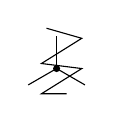
\begin{tikzpicture}[scale=.64]\fill(0,0)circle(2pt);\draw(0,0)--(90:.65);\draw(0,0)--(210:.65);\draw(0,0)--(330:.65);\draw(-.2,.8)--(.5,.6)--(-.3,.1)--(.5,0)--(-.3,-.5)--(.2,-.5);\end{tikzpicture}}}
\[\left(\begin{smallmatrix}3\\1_3\end{smallmatrix},2_3,6\right)\]
h) $3$ sommets d’ordre $2$
\figure{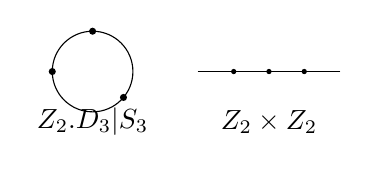
\begin{tikzpicture}[scale=.64,line cap=round,line join=round]\begin{scope}[shift={(0,0)}]\draw(0,0)circle(.8);\foreach\a in{90,180,320}\fill(\a:.8)circle(2pt);\node at(0,-1){$\uline{\mathbb Z_2.\unsure{D_3|\mathfrak S_3}}$};\end{scope}\begin{scope}[shift={(3.5,0)}]\draw(-1.4,0)--(1.4,0);\foreach\x in{-.7,0,.7}\fill(\x,0)circle(1.5pt);\node at(0,-1){$\mathbb Z_2\times\mathbb Z_2$};\end{scope}\end{tikzpicture}}
\margin{$\left(2_3,2_3,3_2\right)$\\$\left(2_3,\begin{smallmatrix}2_2\\1_2\end{smallmatrix},6\right)$}
i) $2$ sommets d’ordre $2$, $2$ d’ordre $1$
\figure{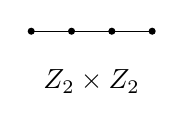
\begin{tikzpicture}[scale=.64,line cap=round,line join=round]\begin{scope}[shift={(0,0)}]\draw(-1.2,0)--(1.2,0);\foreach\x in{-1.2,-.4,.4,1.2}\fill(\x,0)circle(2pt);\node at(0,-1){$\mathbb Z_2\times\mathbb Z_2$};\end{scope}\end{tikzpicture}}
\[\left(\begin{smallmatrix}2_2\\1_2\end{smallmatrix},2_3,6\right)\]
j) $1$ sommet d’ordre $2$, $4$ d’ordre $1$
\figure{\begin{tikzpicture}\draw(0,0)--(.9,0);\fill(0,0)circle(1pt);\fill(.9,0)circle(1pt);\node[draw,ellipse]at(3,.3){impossible};\end{tikzpicture}}
